%\documentclass[graphics,14pt]{beamer}
%\geometry{papersize={338.7mm,190.5mm},margin={1.125cm,0.125cm}}
%\usepackage[utf8]{inputenc}
%\usepackage[brazil]{babel}
%\usetheme{boxes}
%\usepackage[sfdefault]{carlito}
%\usepackage{natbib}
%% -----------------------------------------------------------------------
%% --- Slide Justificado -------------------------------------------------
%\usepackage{ragged2e}
%\usepackage{etoolbox}
%\usepackage{scrextend} % ajustar texto para direita
%\usepackage{soulutf8}
%\usepackage[normalem]{ulem}
%\usepackage{cancel}
%\usepackage{bm}
%\usepackage{array}
%\usepackage{wrapfig} 
%\apptocmd{\frame}{}{\justifying}{} % Allow optional arguments after frame.
%\usepackage{amsmath,mathtools}
%\usepackage{verbatim}
%\usepackage{tabularx}
%% -----------------------------------------------------------------------
%% separação entre colunas e linhas de tabelas
%\setlength{\tabcolsep}{0.5cm}
%\renewcommand{\arraystretch}{1}
%% -----------------------------------------------------------------------
%% --- Define a centralização de coluna com largura {|C{1 cm}|}
%\newcolumntype{C}[1]{>{\centering\let\newline\\\arraybackslash\hspace{0pt}}m{#1}}
%\newcolumntype{L}[1]{>{\raggedright\let\newline\\\arraybackslash\hspace{0pt}}m{#1}}
%% -----------------------------------------------------------------------
%\newcommand\litem[1]{\item{\bfseries #1 }}
%
%% --- Letras e simbolos matemáticos -------------------------------------
%% ------------------------------------------------------------------------
%\usepackage{multicol}
%\usepackage{multimedia}
%\usepackage[]{graphicx}
%\usepackage[]{color}
%\usepackage{geometry}
%\usepackage{tabularx}
%\usepackage{gensymb}
%
%% ------------------------------------------------------------------------
%
%% --- Esta definicao deve vir antes --------------------------------------
%\usepackage{graphicx}			% Inclusão de gráficos
%\usepackage{float}  
%% ------------------------------------------------------------------------
%\usefonttheme[onlymath]{serif}
%\usepackage{hyperref}
%\usepackage{breakurl}
%\usepackage{multirow}
%\usepackage{subfig}
%\usepackage{ragged2e}
%%\captionsetup[subfigure]{labelformat=empty}
%\usepackage{color}
%\usepackage{colortbl}
%\usepackage{textpos}
%\usepackage{tikz}
%\usetikzlibrary{calc}
%%---------------
%\usepackage{tabularx}
%\usepackage{booktabs}
%\usepackage{multimedia}
%\usepackage[style=british]{csquotes}
%\usepackage{listings}
%
%\renewcommand{\familydefault}{\sfdefault}
%
%% ------------------------------------------------------------------------
%\lstset{language=R,
%	basicstyle=\large\ttfamily,
%	stringstyle=\color{teal},
%	otherkeywords={0,1,2,3,4,5,6,7,8,9},
%	morekeywords={TRUE,FALSE},
%	deletekeywords={data,frame,length,as,character},
%	keywordstyle=\color{blue},
%	commentstyle=\color{teal},
%	showspaces=false,               % show spaces adding particular underscores
%	showstringspaces=false,         % underline spaces within strings
%	showtabs=false,                 % show tabs within strings adding particular underscores
%%	frame=single,                   % adds a frame around the code
%	tabsize=1,                      % sets default tabsize to 2 spaces
%	captionpos=b,                   % sets the caption-position to bottom
%	breaklines=true,                % sets automatic line breaking
%	breakatwhitespace=false, 
%}
%% ------------------------------------------------------------------------
%\pdfsuppresswarningpagegroup=1
%\def\disciplina/{Aplicação da Linguística Computacional nas Ciências Forenses}
%% ------------------------------------------------------------------------
%\tikzset{
%	invisible/.style={opacity=0},
%	visible on/.style={alt={#1{}{invisible}}},
%	alt/.code args={<#1>#2#3}{%
%		\alt<#1>{\pgfkeysalso{#2}}{\pgfkeysalso{#3}} % \pgfkeysalso doesn't change the path
%	},
%}
%% ------------------------------------------------------------------------
%\def\signed #1{{\leavevmode\unskip\nobreak\hfil\penalty50\hskip1em
%		\hbox{}\nobreak\hfill #1%
%		\parfillskip=0pt \finalhyphendemerits=0 \endgraf}}
%\newsavebox\mybox
%\newenvironment{aquote}[1]
%{\savebox\mybox{#1}\begin{quote}}
%	{\vspace*{1mm}\signed{\usebox\mybox}\end{quote}}
%% ------------------------------------------------------------------------
%% --- Desativando os botoes de navegacao ---------------------------------
%\setbeamertemplate{navigation symbols}{}
%% ------------------------------------------------------------------------
%% --- Tela cheia ---------------------------------------------------------
%\hypersetup{pdfpagemode=FullScreen}
%% ------------------------------------------------------------------------
%% --- Layout da pagina ---------------------------------------------------
%\hypersetup{pdfpagelayout=SinglePage}
%% ------------------------------------------------------------------------
%% --- Relaxed footnotes --------------------------------------------------
%\newcommand{\lfr}[1]{\let\thefootnote\relax\footnote{\hspace{0.6cm}\vspace{1.25cm} #1}}
%% --- Pasta com as imagens -----------------------------------------------
%\graphicspath{{Imagens/}}
%% --- Define o cinza tema ------------------------------------------------
%\definecolor{pcmggray}{rgb}{0.5, 0.5, 0.5}
%% --- Define o estilo do titulo do frame ---------------------------------
%\setbeamertemplate{frametitle}{ 
%	\Huge{\bfseries{\insertframetitle\par}\vskip-18pt\hrulefill}
%	\begin{tikzpicture}[remember picture,overlay]
%	\node[xshift=0.65cm,yshift=-1.28 cm,opacity=1.0] at (current page.north west) {\includegraphics[width=0.56cm]{00BAS_marcador_02.pdf}};
%	\end{tikzpicture}
%}
%%\multicolbaselineskip = 1cm
% \columnsep = 1cm
%% ------------------------------------------------------------------------
%\setbeamercolor{frametitle}{fg=pcmggray,bg=white}
%\setbeamerfont{structure}{size=\LARGE}
%\setbeamerfont{itemize/enumerate body}{size=\LARGE}
%\setbeamerfont{itemize/enumerate subbody}{size=\LARGE}
%\setbeamerfont{normal text}{size=\LARGE}
%\setbeamercolor{structure}{fg=black} % itemize, enumerate, etc
%\setbeamercolor{section in toc}{fg=black} % TOC sections
%\setbeamertemplate{bibliography item}{}
%\setbeamerfont{bibliography item}{size=\normalsize}
%\setbeamerfont{bibliography entry author}{size=\normalsize}
%\setbeamerfont{bibliography entry title}{size=\normalsize,series=\bfseries}
%\setbeamerfont{bibliography entry location}{size=\normalsize}
%\setbeamerfont{bibliography entry note}{size=\normalsize}
%\AtBeginDocument{\usebeamerfont{normal text}}
%% --- Fundo da pagina de titulo ------------------------------------------
%\setbeamertemplate{background} 
%{
%	\begin{tikzpicture}[remember picture, overlay]
%	\node[xshift=5.75cm,yshift=-1.68cm,opacity=1.0] at (current page.north west) {\includegraphics[width=11.49cm]{00BAS_titleleftupimage.pdf}};
%	\node[xshift=16.93cm,yshift=-6.47cm,opacity=1.0] at (current page.north west) {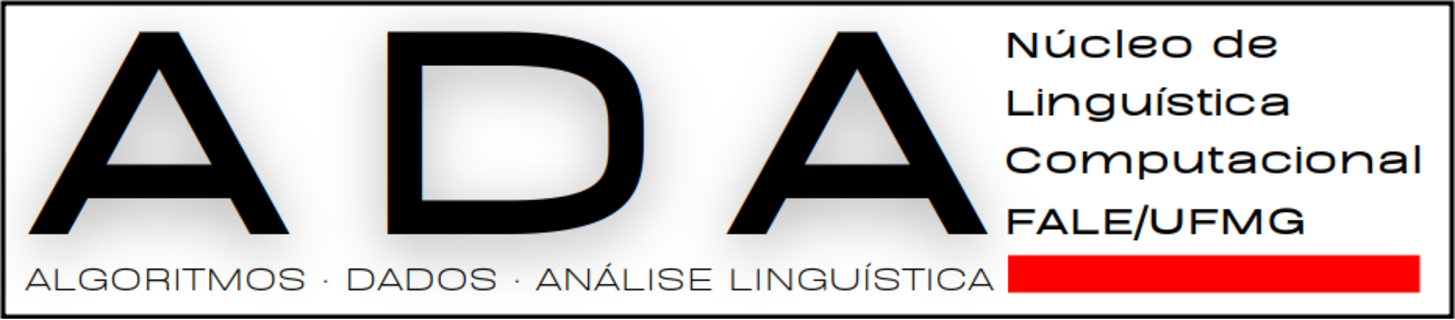
\includegraphics[width=18.0cm]{00BAS_ada_ufmg.pdf}};
%	\node[xshift=28.35cm,yshift=-17.48cm,opacity=1.0] at (current page.north west) {\includegraphics[width=11.04cm]{00BAS_titlerightdown.pdf}};
%	\end{tikzpicture}
%}
%% ------------------------------------------------------------------------
%\defbeamertemplate*{title page}{customized}[1][]
%{
%	\begin{center}
%	\vspace{-1.5cm}
%	\usebeamerfont{title}\LARGE{\textbf{\inserttitle}}\par
%	\vspace{9cm}
%	\usebeamerfont{subtitle}\huge{\textbf{\insertsubtitle}}\par
%	\vspace{2cm}
%	\usebeamerfont{author}\textbf{\insertauthor}\par
%	\end{center}
%	\vfill
%}
%\title{Um Convite para a Linguística Computacional}
%\subtitle{\disciplina/}
%\author[Silva, A. P.]{Adelino Pinheiro Silva}
%\date{\today}
%% =======================================================================
%% INICIO DO CONTEUDO PRINCIPAL
%% =======================================================================
%\begin{document}
% \frame{\titlepage}
% =======================================================================
% ---- Fundo da demais paginas ------------------------------------------
%\setbeamertemplate{background} 
%{
%	\begin{tikzpicture}[remember picture, overlay]
%	\node[xshift=1.14cm,yshift=-17.88cm,opacity=1.0] at (current page.north west) {
\includegraphics[width=1.58cm]{00BAS_fale_logo.pdf}};
%	\node[xshift=28.97cm,yshift=-18.2cm,opacity=1.0] at (current page.north west) {\includegraphics[width=9.8cm]{00BAS_regularrightdown.pdf}};
%	\end{tikzpicture}
%	\put(880,-20){\Large{\insertframenumber \hspace{2pt} de \inserttotalframenumber}}
%%	\begin{textblock}{2cm}(150pt,1pt)
%%		\normalsize \insertframenumber de \inserttotalframenumber
%%	\end{textblock}
%%	\normalsize \insertframenumber de \inserttotalframenumber
%}
%\documentclass[graphics,14pt]{beamer}
%\geometry{papersize={338.7mm,190.5mm},margin={1.125cm,0.125cm}}
\documentclass[121pt, aspectratio=169, t]{beamer}
\usepackage[utf8]{inputenc}
\usepackage[brazil]{babel}
\usepackage{beamerthemesplit}

%-----------------------------------------------------------------------------------------------
% --- Slide Justificado --------------------------------------------------------------
\usepackage{ragged2e}
\usepackage{etoolbox}
\usepackage{soul}
\usepackage[normalem]{ulem}
\usepackage{cancel}
\usepackage{bm}
\usepackage{array}
\usepackage{wrapfig} 
\apptocmd{\frame}{}{\justifying}{} % Allow optional arguments after frame.
\usepackage{amsmath,mathtools}
\usepackage{scrextend} % ajustar texto para direita
%\usepackage{enumitem}
%\usepackage{showframe}
% =============================================================================
% Pacotes para simbolos IPA
% =============================================================================
\usepackage{tipa}		% Simbolos do IPA
\usepackage{tipx}
%-----------------------------------------------------------------------------------------------
% Alguns acronimos - usar ou não
\def\CFL/{CFL}%{comparação forense de locutor}
\def\IntervEst/{estimativa por intervalo}%{inferência intervalar}
%-----------------------------------------------------------------------------------------------
% separação entre colunas e linhas de tabelas
\setlength{\tabcolsep}{2pt}
\renewcommand{\arraystretch}{1}
%-----------------------------------------------------------------------------------------------
% Define a centralização de coluna com largura {|C{1 cm}|}
\newcolumntype{C}[1]{>{\centering\let\newline\\\arraybackslash\hspace{0pt}}m{#1}}
\newcolumntype{L}[1]{>{\raggedright\let\newline\\\arraybackslash\hspace{0pt}}m{#1}}
%-----------------------------------------------------------------------------------------------
\newcommand\litem[1]{\item{\bfseries #1 }}
% --- Configuracoes de Tema e cores --------------------------------------------------
\usetheme{CambridgeUS}

\definecolor{darkblue}{rgb}{0.07058,0.06470,0.01176}  % Preto 		RGB 21,20,16
\definecolor{yellow}{rgb}{0.57058,0.66470,0.71176} 	
\definecolor{myred}{rgb}{0.808,0.086,0.133}   % 0.98823,0.00000,0.00784
% amarelo	RGB (1,1,0.588224) 255,255,150 PAULA 4
\definecolor{myblue}{rgb}{0.57058,0.66470,0.71176} % azul 	RGB 13,29,174

\setbeamercolor{item}{fg=myblue}

\setbeamercolor{alerted text}{fg=yellow}	
\setbeamercolor*{palette primary}{fg=darkblue,bg=yellow}
\setbeamercolor*{palette secondary}{fg=darkblue,bg=myred}
\setbeamercolor*{palette tertiary}{bg=darkblue,fg=yellow}
\setbeamercolor*{palette quaternary}{fg=darkblue,bg=yellow}

\setbeamercolor*{sidebar}{fg=darkblue,bg=orange!75!white}

\setbeamercolor*{palette sidebar primary}{fg=darkblue}
\setbeamercolor*{palette sidebar secondary}{fg=white}
\setbeamercolor*{palette sidebar tertiary}{fg=white} % darkblue!50!black
\setbeamercolor*{palette sidebar quaternary}{fg=white} % yellow!10!orange

\setbeamercolor*{titlelike}{parent=palette primary}
\setbeamercolor{frametitle}{bg=yellow}
\setbeamercolor{frametitle right}{bg=yellow}

\setbeamercolor*{separation line}{bg=myblue}
\setbeamercolor*{fine separation line}{bg=myblue}


% --- Letras e simbolos matemáticos --------------------------------------------------
% ------------------------------------------------------------------------------------
\usepackage[bbgreekl]{mathbbol}  % Pacote para repreentação de conjuntos com \mathbb{R} com letras gregas
\usepackage{amsfonts}	% Pacote para repreentação de conjuntos com \mathbb{R}
\usepackage{mathrsfs}	% Pacote para letras matemáticas

\usepackage{amssymb} 	% diversos simbolos matematicos adicionais. Carrega automático com amsfonts
% ------------------------------------------------------------------------------------
\usepackage{multicol}

\usepackage{multimedia}
\usepackage[]{graphicx}
\usepackage[]{color}
\usepackage{geometry}
\usepackage{media9}

\usepackage{tabularx}
\usepackage{amsmath, amsthm, amssymb}
\usepackage{gensymb}

% ------------------------------------------------------------------------------------

% --- Esta definicao deve vir antes --------------------------------------------------
\usepackage{graphicx}			% Inclusão de gráficos
\usepackage{float}  
% ------------------------------------------------------------------------------------
\usefonttheme[onlymath]{serif}
\usepackage{hyperref}
\usepackage{multirow}
\usepackage{subfig}
\usepackage{ragged2e}
\captionsetup[subfigure]{labelformat=empty}
\usepackage{color}
\usepackage{colortbl}
\usepackage{textpos}
\usepackage{tikz}
\usetikzlibrary{calc}
%---------------
\usepackage{tabularx}
\usepackage{booktabs}

\usepackage{multimedia}

%\newenvironment{leftbox}[1]
%{\itemize[
%	nosep,
%	leftmargin=0pt,
%	rightmargin=\dimexpr\textwidth-#1\relax,
%	itemindent=\parindent,
%	listparindent=\parindent,
%	]\item[]\relax}
%{\enditemize}
%
%\newenvironment{rightbox}[1]
%{\itemize[
%	nosep,
%	leftmargin=\dimexpr\textwidth-#1\relax,
%	rightmargin=0pt,
%	itemindent=\parindent,
%	listparindent=\parindent,
%	]\item[]\relax}
%{\enditemize}


\tikzset{
	invisible/.style={opacity=0},
	visible on/.style={alt={#1{}{invisible}}},
	alt/.code args={<#1>#2#3}{%
		\alt<#1>{\pgfkeysalso{#2}}{\pgfkeysalso{#3}} % \pgfkeysalso doesn't change the path
	},
}

\newenvironment{caixadireita}[2][.5\linewidth]
{\par\hfill\tabular{@{}p{#1}@{}}
	\multicolumn{1}{@{}c@{}}{#2} \\ }
{\endtabular\par}

% --- Desativando os botoes de navegacao ---------------------------------------------
\setbeamertemplate{navigation symbols}{}
% ------------------------------------------------------------------------------------
% --- Tela cheia ---------------------------------------------------------------------
\hypersetup{pdfpagemode=FullScreen}
% ------------------------------------------------------------------------------------
% --- Layout da pagina ---------------------------------------------------------------
\hypersetup{pdfpagelayout=SinglePage}
% ------------------------------------------------------------------------------------
% --- Relaxed footnotes --------------------------------------------------------------
\newcommand{\lfr}[1]{\let\thefootnote\relax\footnote{\tiny #1}}
% --- Pasta com as imagens -----------------------------------------------------------
\graphicspath{{Imagens/}}
\DeclareMathOperator{\erf}{erf}
% ------------------------------------------------------------------------------------
\title[Linguística Computacional]{Aplicação da Linguística Computacional nas Ciências Forenses}
\author[Silva, A. P.]{Adelino Pinheiro Silva\vspace{0cm}}
\institute[ADA]{ \footnotesize{Núcleo de Linguística Computacional (ADA) \\ Faculade de Letras (FALE) \\ Universidade Federal de Minas Gerais (UFMG)} \\ \vspace{0cm}}
\date{\today}

\begin{document}
	\begin{tikzpicture}[remember picture,overlay]
		\node[xshift=-4.5cm,yshift=-3.25cm,opacity=1.0] at (current page.center) {
\includegraphics[width=6cm]{ADA_logo-borda.png}};
	\end{tikzpicture}
	\frame{\titlepage}
	
	
% =======================================================================================
	
% ==== Sumário ==========================================================================
\section{Sumário}
\begin{frame}
	\frametitle{Sumário}
	\tableofcontents
\end{frame}
% =======================================================================================

% =======================================================================================
\AtBeginSection[]
{
	\begin{frame}
		\frametitle{Assuntos}
		\tableofcontents[currentsection]
	\end{frame}
}
% =======================================================================================
\section{Introdução}
\begin{frame}[fragile=singleslide]
	\frametitle{Visão Geral das Ciências Forenses}
	\begin{tikzpicture}[remember picture,overlay]
		\node[xshift=0cm,yshift=-0.5cm,opacity=1.0] at (current page.center) {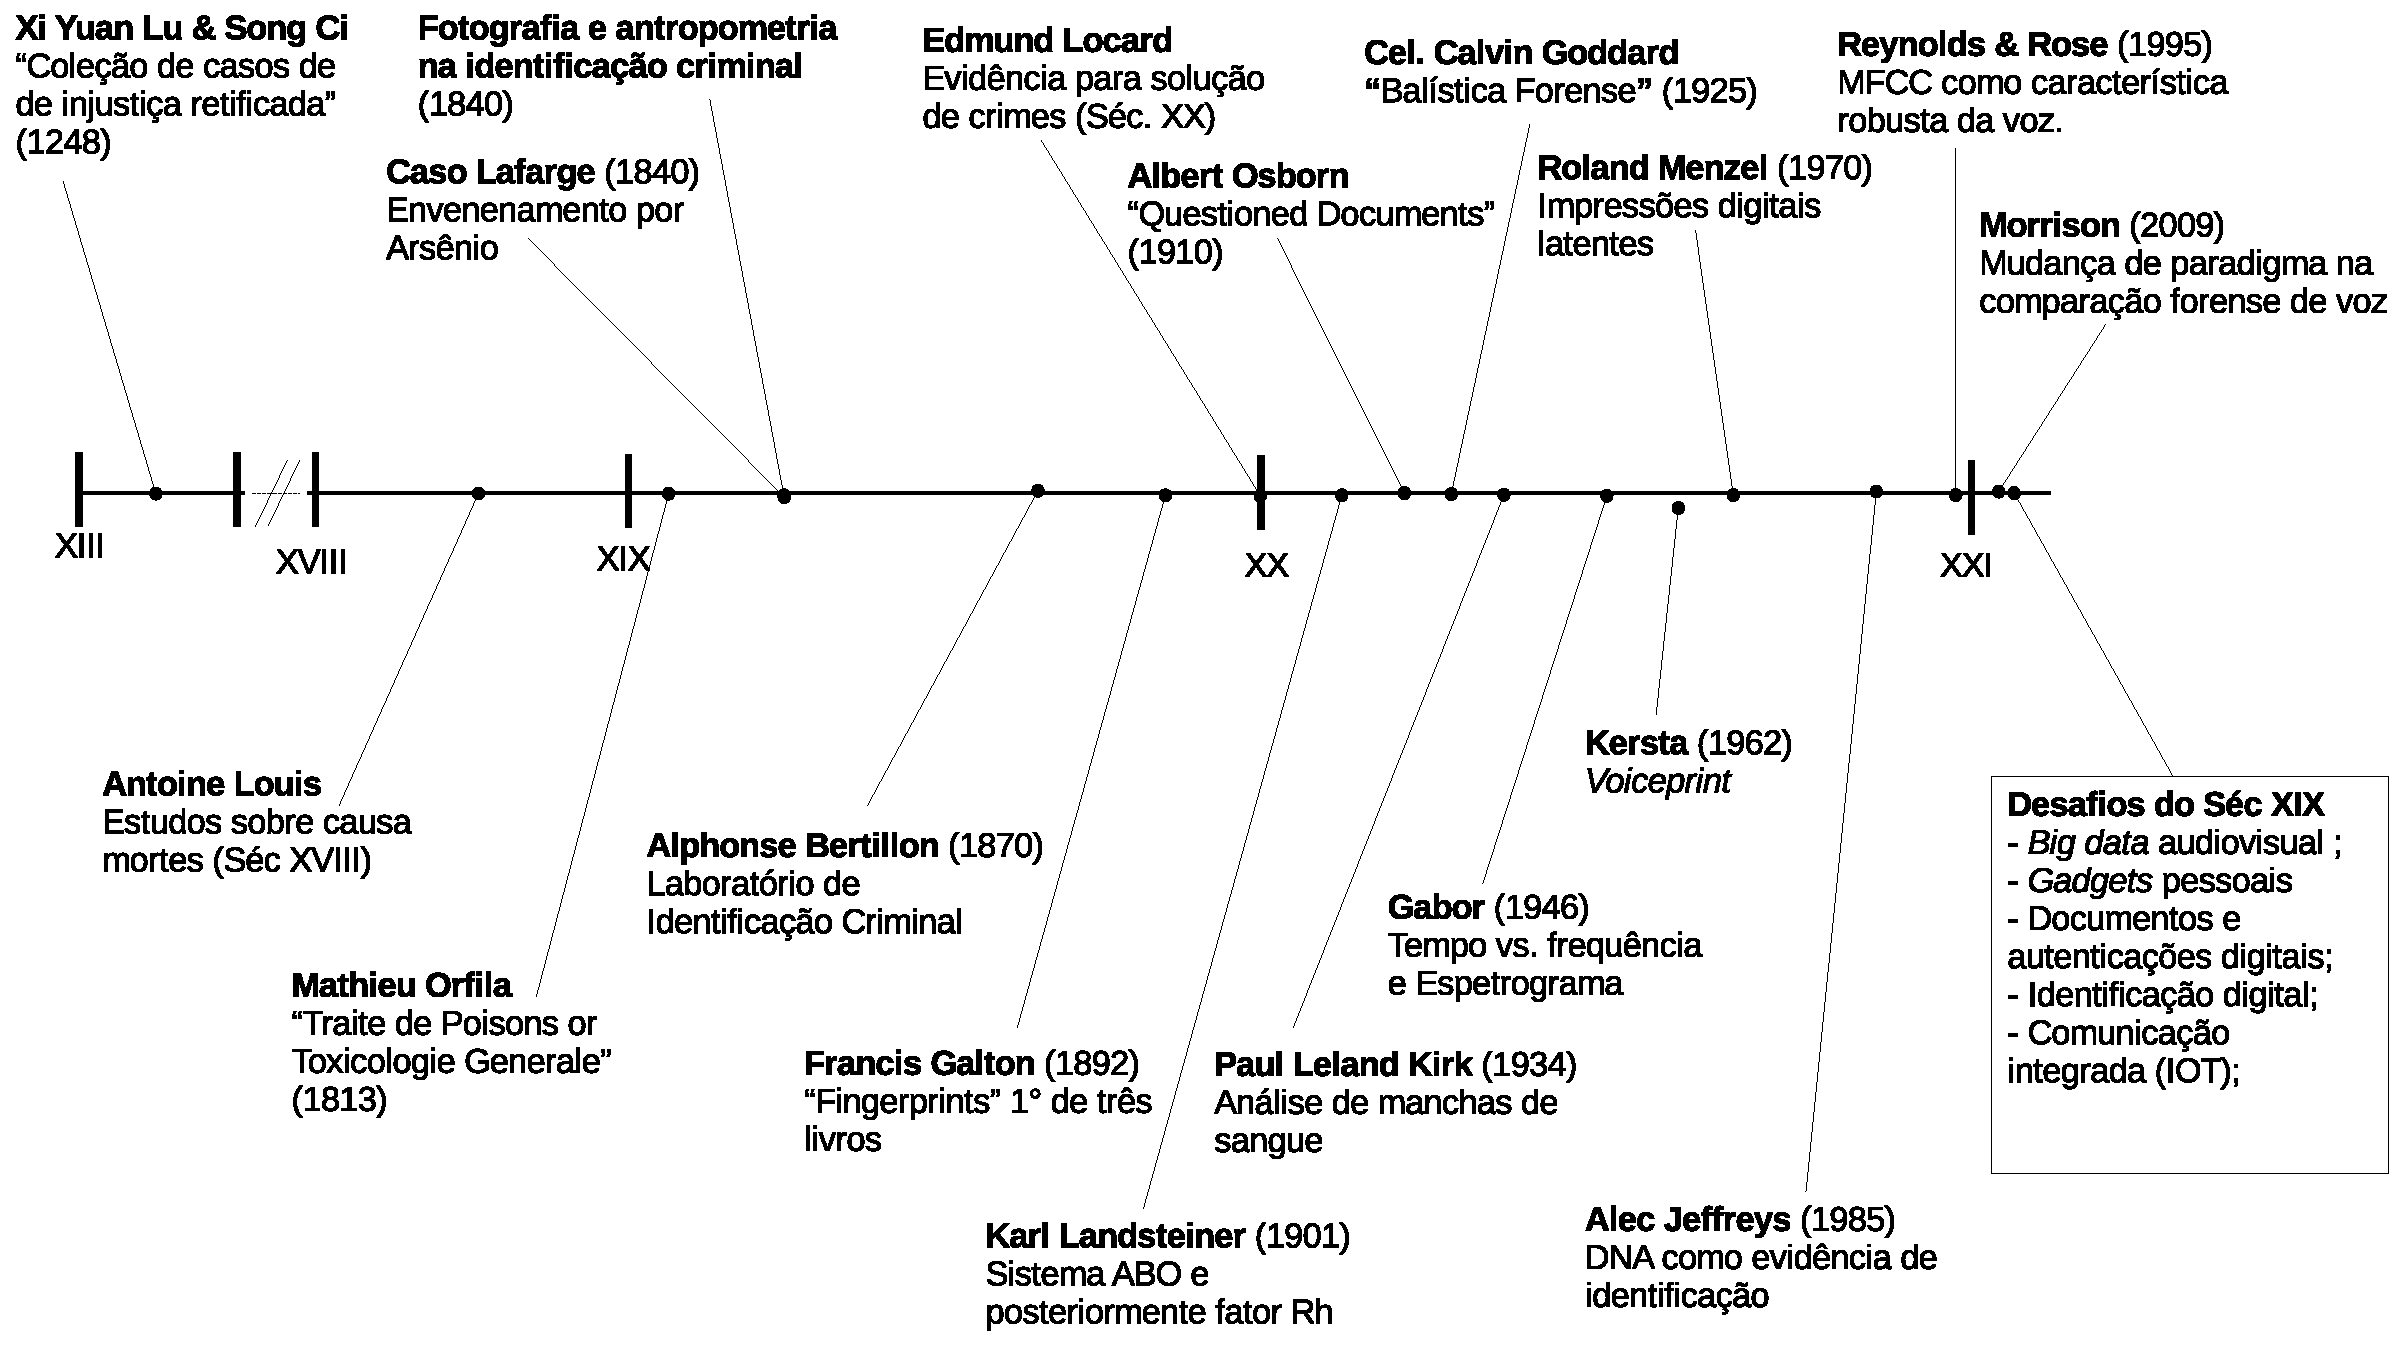
\includegraphics[width=13cm]{Diagrama_Historia_Forense.pdf}};
	\end{tikzpicture}
	\vfill
	\lfr{Imagem: {Arquivo do autor.}}
	
\end{frame}

\begin{frame}[fragile=singleslide]
	\frametitle{Visão Geral das Ciências Forenses}
	\begin{itemize}[]
		\item Conjunto de conhecimentos e técnicas.
		\item Aplicadas a assuntos legais.
		\item Livro Xi Yuan Lu (Registro de injustiça \\ ou lavagem dos erros).
		\item Escola alemã \textit{Kriminalistik}.
		\item Escola Francesa Locard.
%		\item 
	\end{itemize}
	\vspace{0.75cm}
	\begin{itemize}[]
		\item Arquimedes, Poincaré, 
		\item Conan Doyle, Maurice Leblanc, Barry Allen.
	\end{itemize}

	\begin{tikzpicture}[remember picture,overlay]
		\node[xshift=4.75cm,yshift=0.5cm,opacity=1.0] at (current page.center) {\includegraphics[width=6cm]{Foto-Henrique-Almeida-11.jpg}};
	\end{tikzpicture}
	\vfill
	\lfr{Imagem: \url{https://noticias.paginas.ufsc.br/files/2022/09/Foto-Henrique-Almeida-11.jpg}}
	
\end{frame}

% ------------------------------------------------------------------------
\section{Linguística Computacional Forense}
\begin{frame}[fragile=singleslide]
	\frametitle{Definição}
	
	\begin{caixadireita}[.8\linewidth]{}
		``\textit{a parte da ciência linguística que se preocupa com o 	tratamento computacional da linguagem, e sua aplicações}.'' \\ \hspace*{\fill}Gabriel de Ávila Othero.
	\end{caixadireita}
	\vspace{0.5cm}
	
	\begin{itemize}[]
	\item escritos e manuscritos;
	\item entrevistas de testemunhas vulneráveis no sistema legal;
	\item atribuição de autoria, plágio, edição e manipulação;
	\item fonética forense e identificação do locutor;
	\item fala para texto e traduções;
	\item localização sociolinguística de falantes;
	\item imagem para texto.
	\end{itemize}	
\end{frame}
% ------------------------------------------------------------------------
\begin{frame}[fragile=singleslide]
	\frametitle{Na prática}
	
	\begin{tikzpicture}[remember picture,overlay]
		\node[xshift=3cm,yshift=-1.25cm,opacity=1.0] at (current page.center) {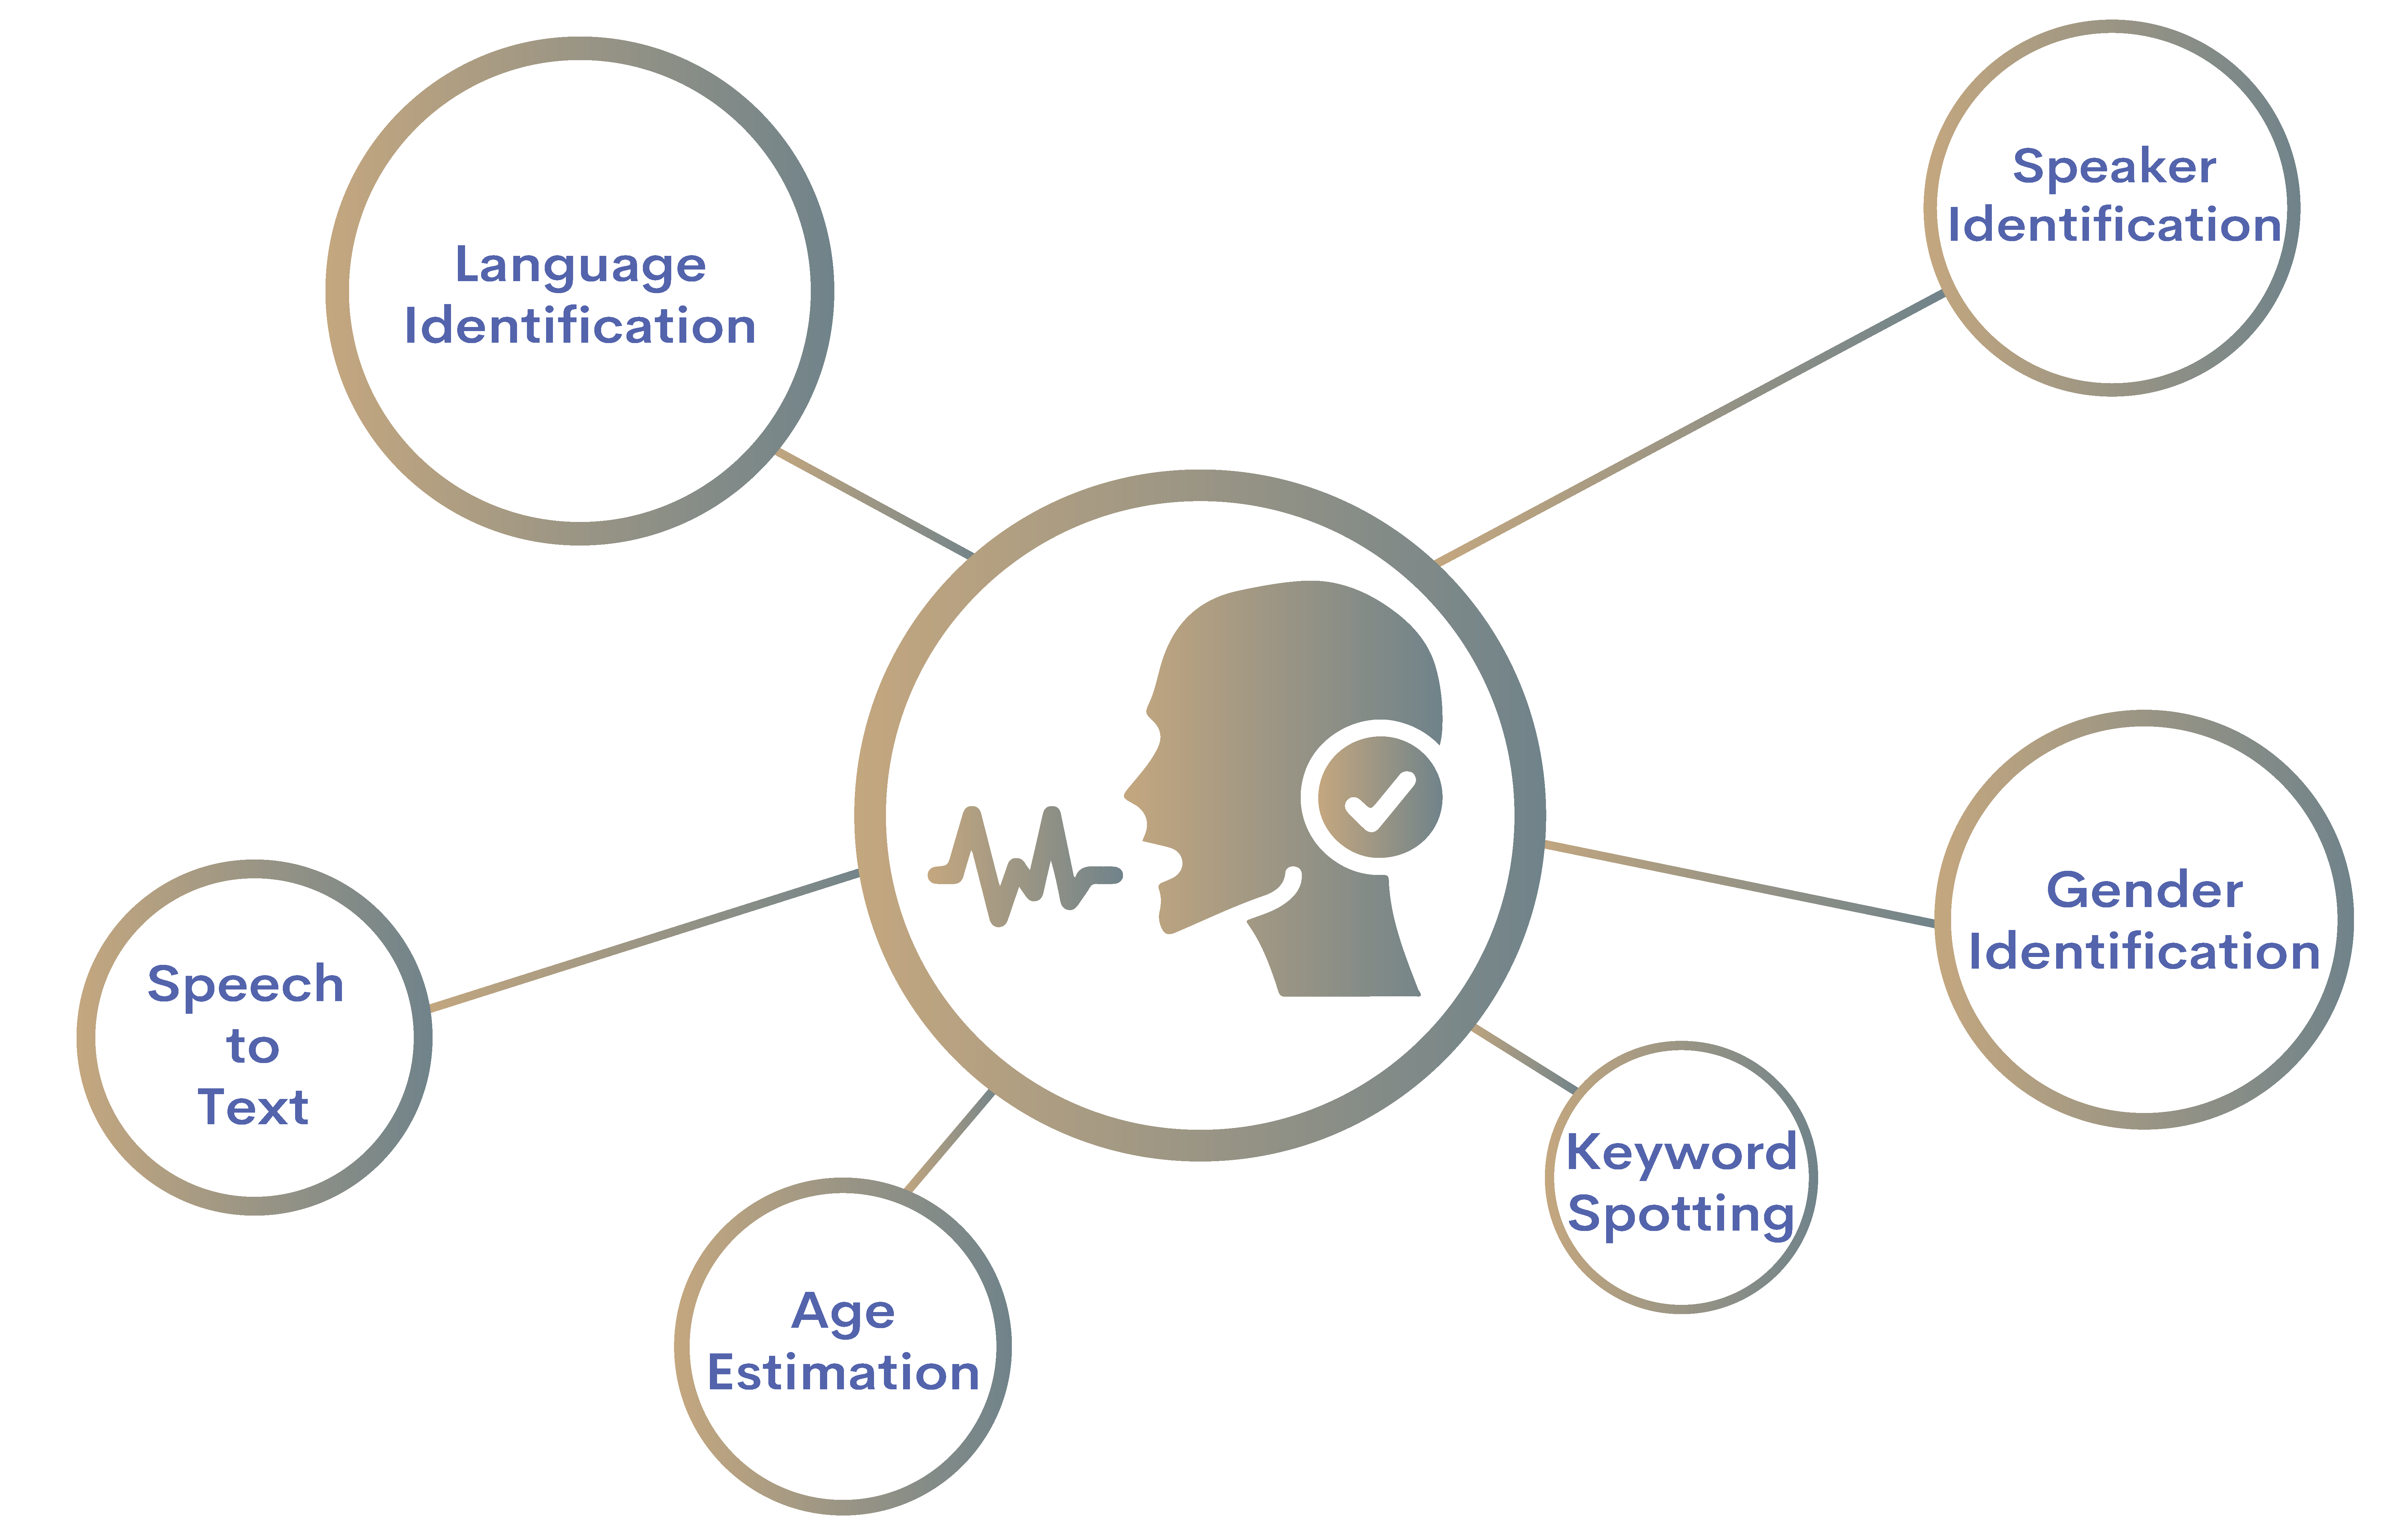
\includegraphics[width=9cm]{f-Voice-FS.png}};
	\end{tikzpicture}\\

	\begin{itemize}[]
		\item corpus;
		\item dados empíricos;
		\item estudos constantes;
		\item NLP; 
		\item programação;
		\item reconhecimento de padrões e estatística.
	\end{itemize}	
	\vfill
	\lfr{Imagem: \url{https://www.stratign.com/voice-forensic-system/}}

\end{frame}
% ------------------------------------------------------------------------
\begin{frame}[fragile=singleslide]
	\frametitle{Escritos e manuscritos}
	
	\vspace{1cm}
	\begin{itemize}[]
		\item grafotécnica
		\item atribuição de estilo.
	\end{itemize}	
	
	\begin{tikzpicture}[remember picture,overlay]
		\node[xshift=3cm,yshift=-0.5cm,opacity=1.0] at (current page.center) {\includegraphics[width=7cm]{carta-filha-metroviario.jpg}};
	\end{tikzpicture}
	
	\vfill
	\lfr{Imagem: \url{https://www.otempo.com.br/cidades/em-carta-filha-de-metroviario-de-bh-faz-apelo-a-lula-salve-os-empregos-1.2885744}}
\end{frame}
% ------------------------------------------------------------------------
\begin{frame}[fragile=singleslide]
	\frametitle{Testemunhas vulneráveis}
	
	\vspace{1cm}
	\begin{itemize}[]
		\item espaço de apoio e acolhimento; 
		\item análise do discursos; 
		\item cuidado com eventos \\ sociais sensíveis.
	\end{itemize}
	
	\begin{tikzpicture}[remember picture,overlay]
		\node[xshift=3cm,yshift=-0.5cm,opacity=1.0] at (current page.center) {\includegraphics[width=8cm]{Depoimento.jpg}};
	\end{tikzpicture}
	\vfill
	\lfr{Imagem: \url{https://www.capistranoadvogados.com.br/images/noticias/grd/119334b48feeb38af04a349145591eb9.jpg}}
\end{frame}
% ------------------------------------------------------------------------
\begin{frame}[fragile=singleslide]
	\frametitle{Plágio, edição e manipulação}
	\vspace{1cm}
	\begin{itemize}[]
		\item reconhecimento de padrões;
		\item música;
		\item atribuição de estilo.
	\end{itemize}

	\begin{tikzpicture}[remember picture,overlay]
		\node[xshift=3cm,yshift=-0.5cm,opacity=1.0] at (current page.center) {\includegraphics[width=5cm]{Traumas_RC.jpg}};
	\end{tikzpicture}
	
	
	\vfill
	\lfr{Imagem: \url{https://genius.com/Roberto-carlos-traumas-lyrics}}
	
\end{frame}
% ------------------------------------------------------------------------
\begin{frame}[fragile=singleslide]
	\frametitle{Localização sociolinguística de falantes}
	
	\begin{tikzpicture}[remember picture,overlay]
		\node[xshift=-3.25cm,yshift=0.cm,opacity=1.0] at (current page.center) {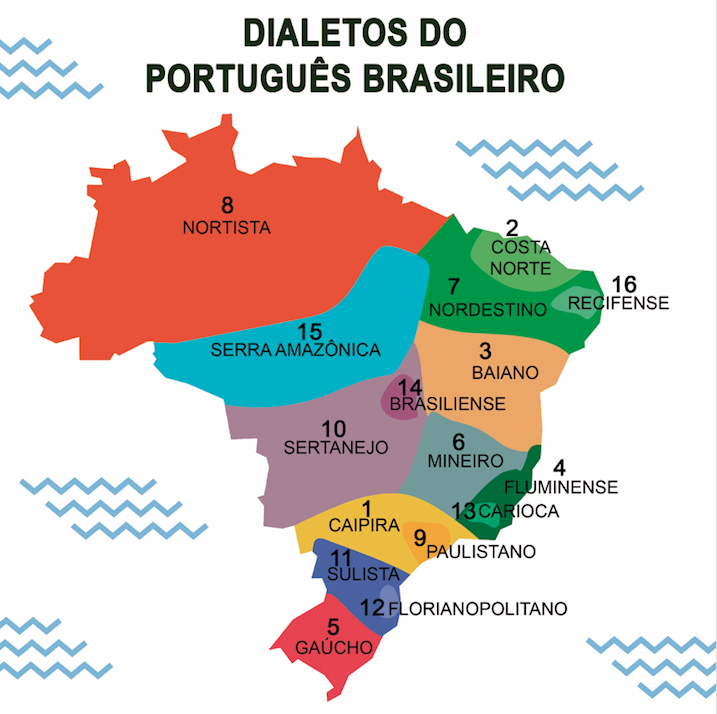
\includegraphics[width=6cm]{captura-de-tela-2019-02-14-as-160635.png}};
	\end{tikzpicture}
	
	\begin{tikzpicture}[remember picture,overlay]
		\node[xshift=3.25cm,yshift=0.0cm,opacity=1.0] at (current page.center) {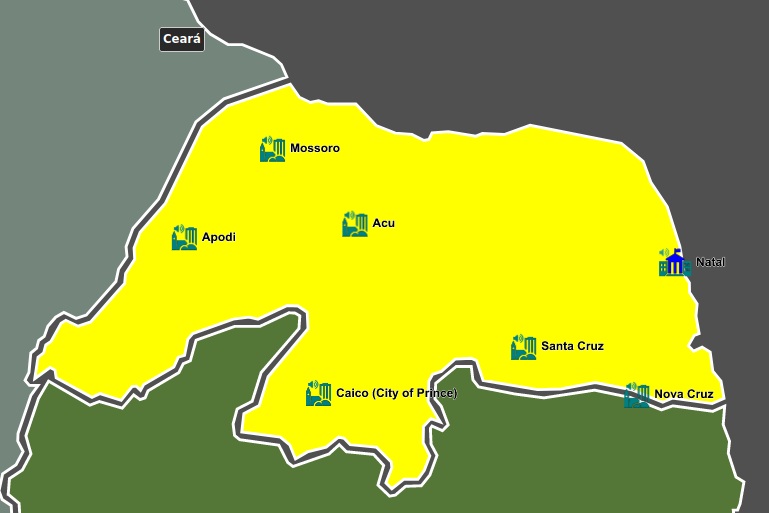
\includegraphics[width=6cm]{Seleção_002.png}};
	\end{tikzpicture}

	\vfill
	\lfr{Imagem: \url{https://localingual.com/} e \url{https://www.thefools.com.br/blog/post/dialetos-do-portugues-brasileiro}}
\end{frame}
% ------------------------------------------------------------------------
\begin{frame}[fragile=singleslide]
	\frametitle{Perspectivas}
	
	Paradigma indutivo:
	\begin{itemize}[]
		\item acúmulo de convergências e divergências;
		\item baseada no material observado; e
		\item difícil inferir sobre a possibilidade de erro.
	\end{itemize}
	
	Paradigma hipotético-dedutivo:
	\begin{itemize}[]
		\item observação são ponderadas pela \\semelhança vs. tipicidade;
		\item necessita de uma base de dados para \\estimação de parâmetros; e
		\item possível estimar erros
	\end{itemize}
	
	\begin{tikzpicture}[remember picture,overlay]
		\node[xshift=4cm,yshift=-0.5cm,opacity=1.0] at (current page.center) {\includegraphics[width=7cm]{Gradiente_descendente.jpg}};
	\end{tikzpicture}

	\vfill
	\lfr{Imagem: \url{https://miro.medium.com/v2/resize:fit:720/format:webp/1*IxMLWG1xsZ50b91M5VJXSA.jpeg}}
\end{frame}
% ------------------------------------------------------------------------
\section{Aplicações da Linguística Computacional nas Ciências Forenses}
\begin{frame}[fragile=singleslide]
	\frametitle{Comparação de Locutor}
	
%	\begin{rightbox}{10cm}
		\begin{itemize}
			\item métodos linguísticos;
			\item medidas acústicas;
		\end{itemize}
%	\end{rightbox}
	
	
	\begin{tikzpicture}[remember picture,overlay]
		\node[xshift=5cm,yshift=0.75cm,opacity=1.0] at (current page.center) {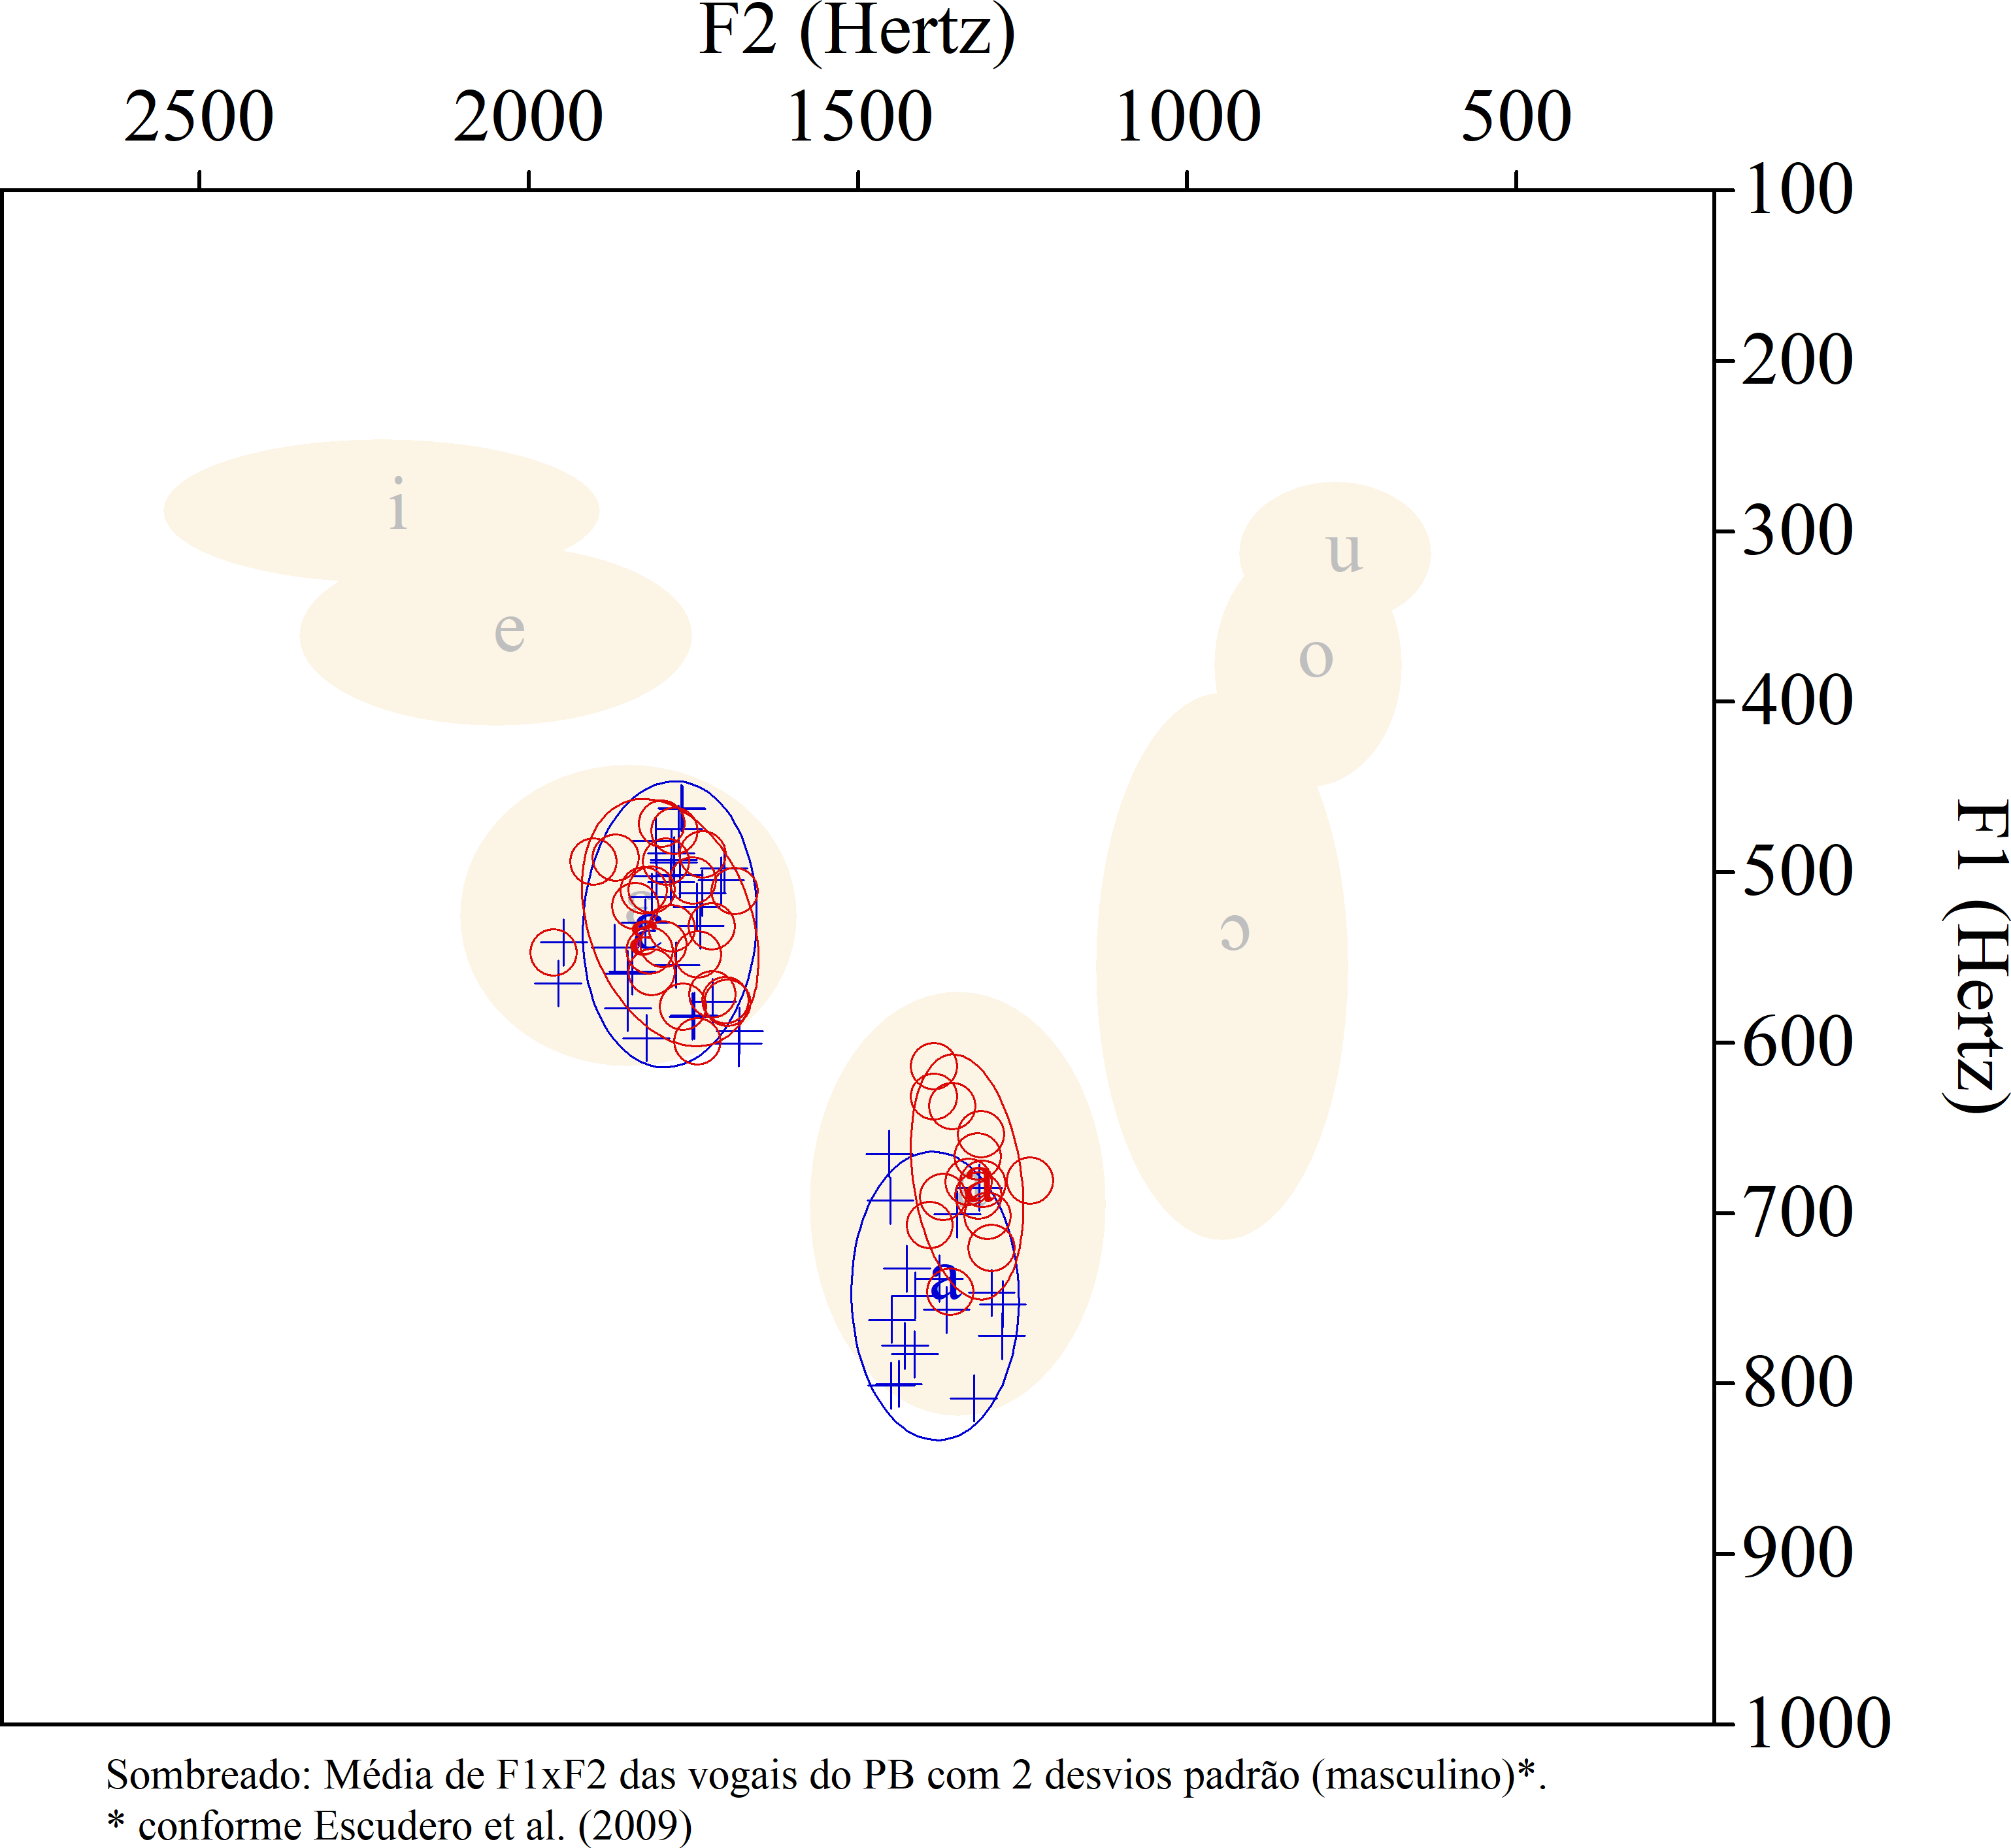
\includegraphics[width=5cm]{Formantes.png}};
	\end{tikzpicture}

	\begin{tikzpicture}[remember picture,overlay]
		\node[xshift=-3.25cm,yshift=-1.15cm,opacity=1.0] at (current page.center) {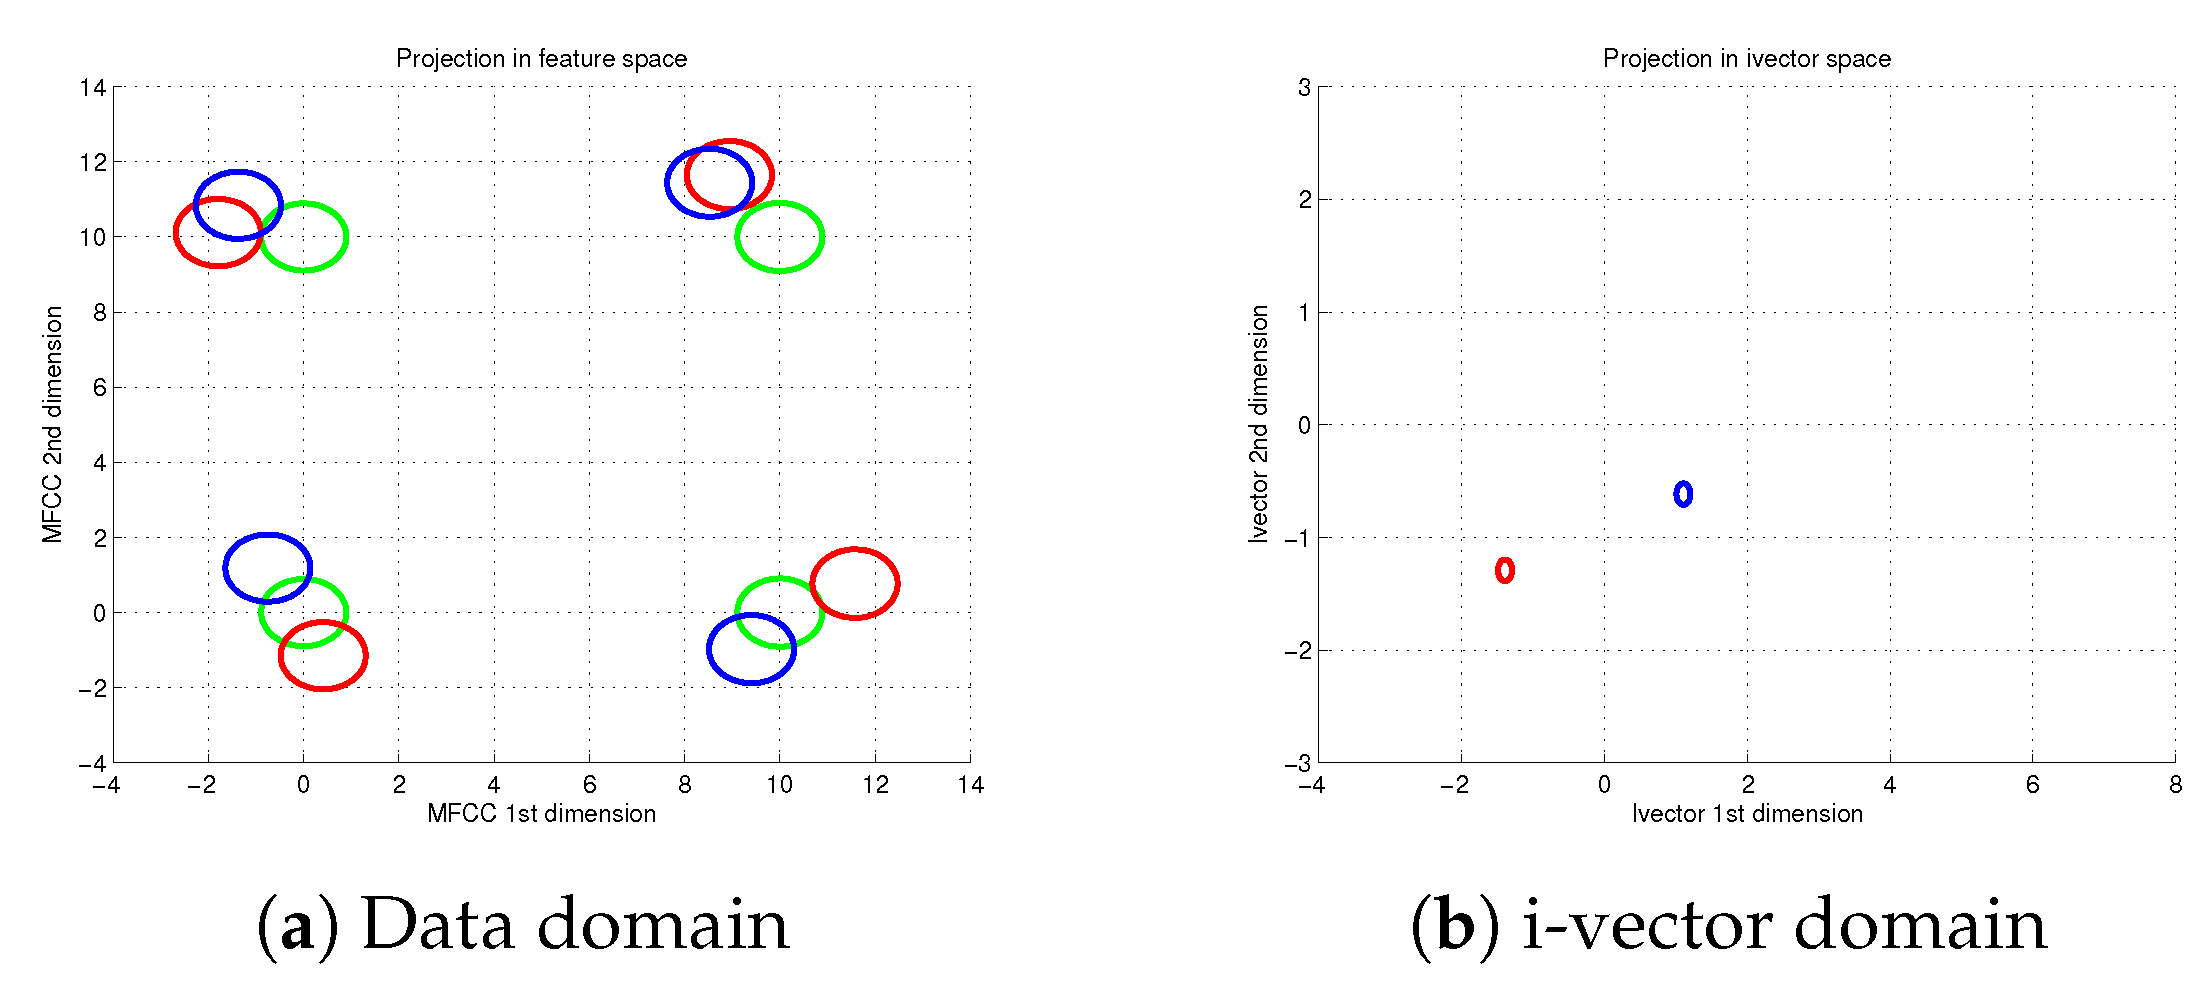
\includegraphics[width=9cm]{projecao_espaco.png}};
	\end{tikzpicture}

	\vfill
	\lfr{Imagem: \url{https://doi.org/10.3390/app9183697} e arquivo pessoal}
\end{frame}
% ------------------------------------------------------------------------
\begin{frame}[fragile=singleslide]
	\frametitle{Interpretação de falas em imagem}
	
	\vspace{1.5cm}
	\begin{itemize}[]
		\item estimar o som da fala a partir \\de pistas articulatórias
		\item taxas de 51\% a 81\%.
	\end{itemize}
	
	\begin{tikzpicture}[remember picture,overlay]
		\node[xshift=3cm,yshift=-0.5cm,opacity=1.0] at (current page.center) {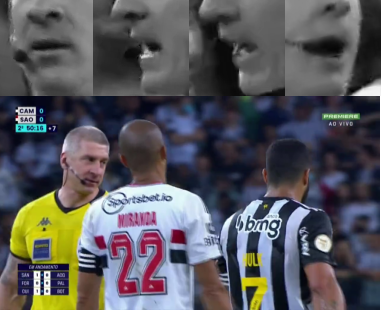
\includegraphics[width=8cm]{CAM_.png}};
	\end{tikzpicture}
	\vfill
	\lfr{Imagem: Arquivo pessoal.}
\end{frame}
% ------------------------------------------------------------------------
\begin{frame}[fragile=singleslide]
	\frametitle{Conversão de áudio em texto}

	\begin{tikzpicture}[remember picture,overlay]
		\node[xshift=0cm,yshift=-0.5cm,opacity=1.0] at (current page.center) {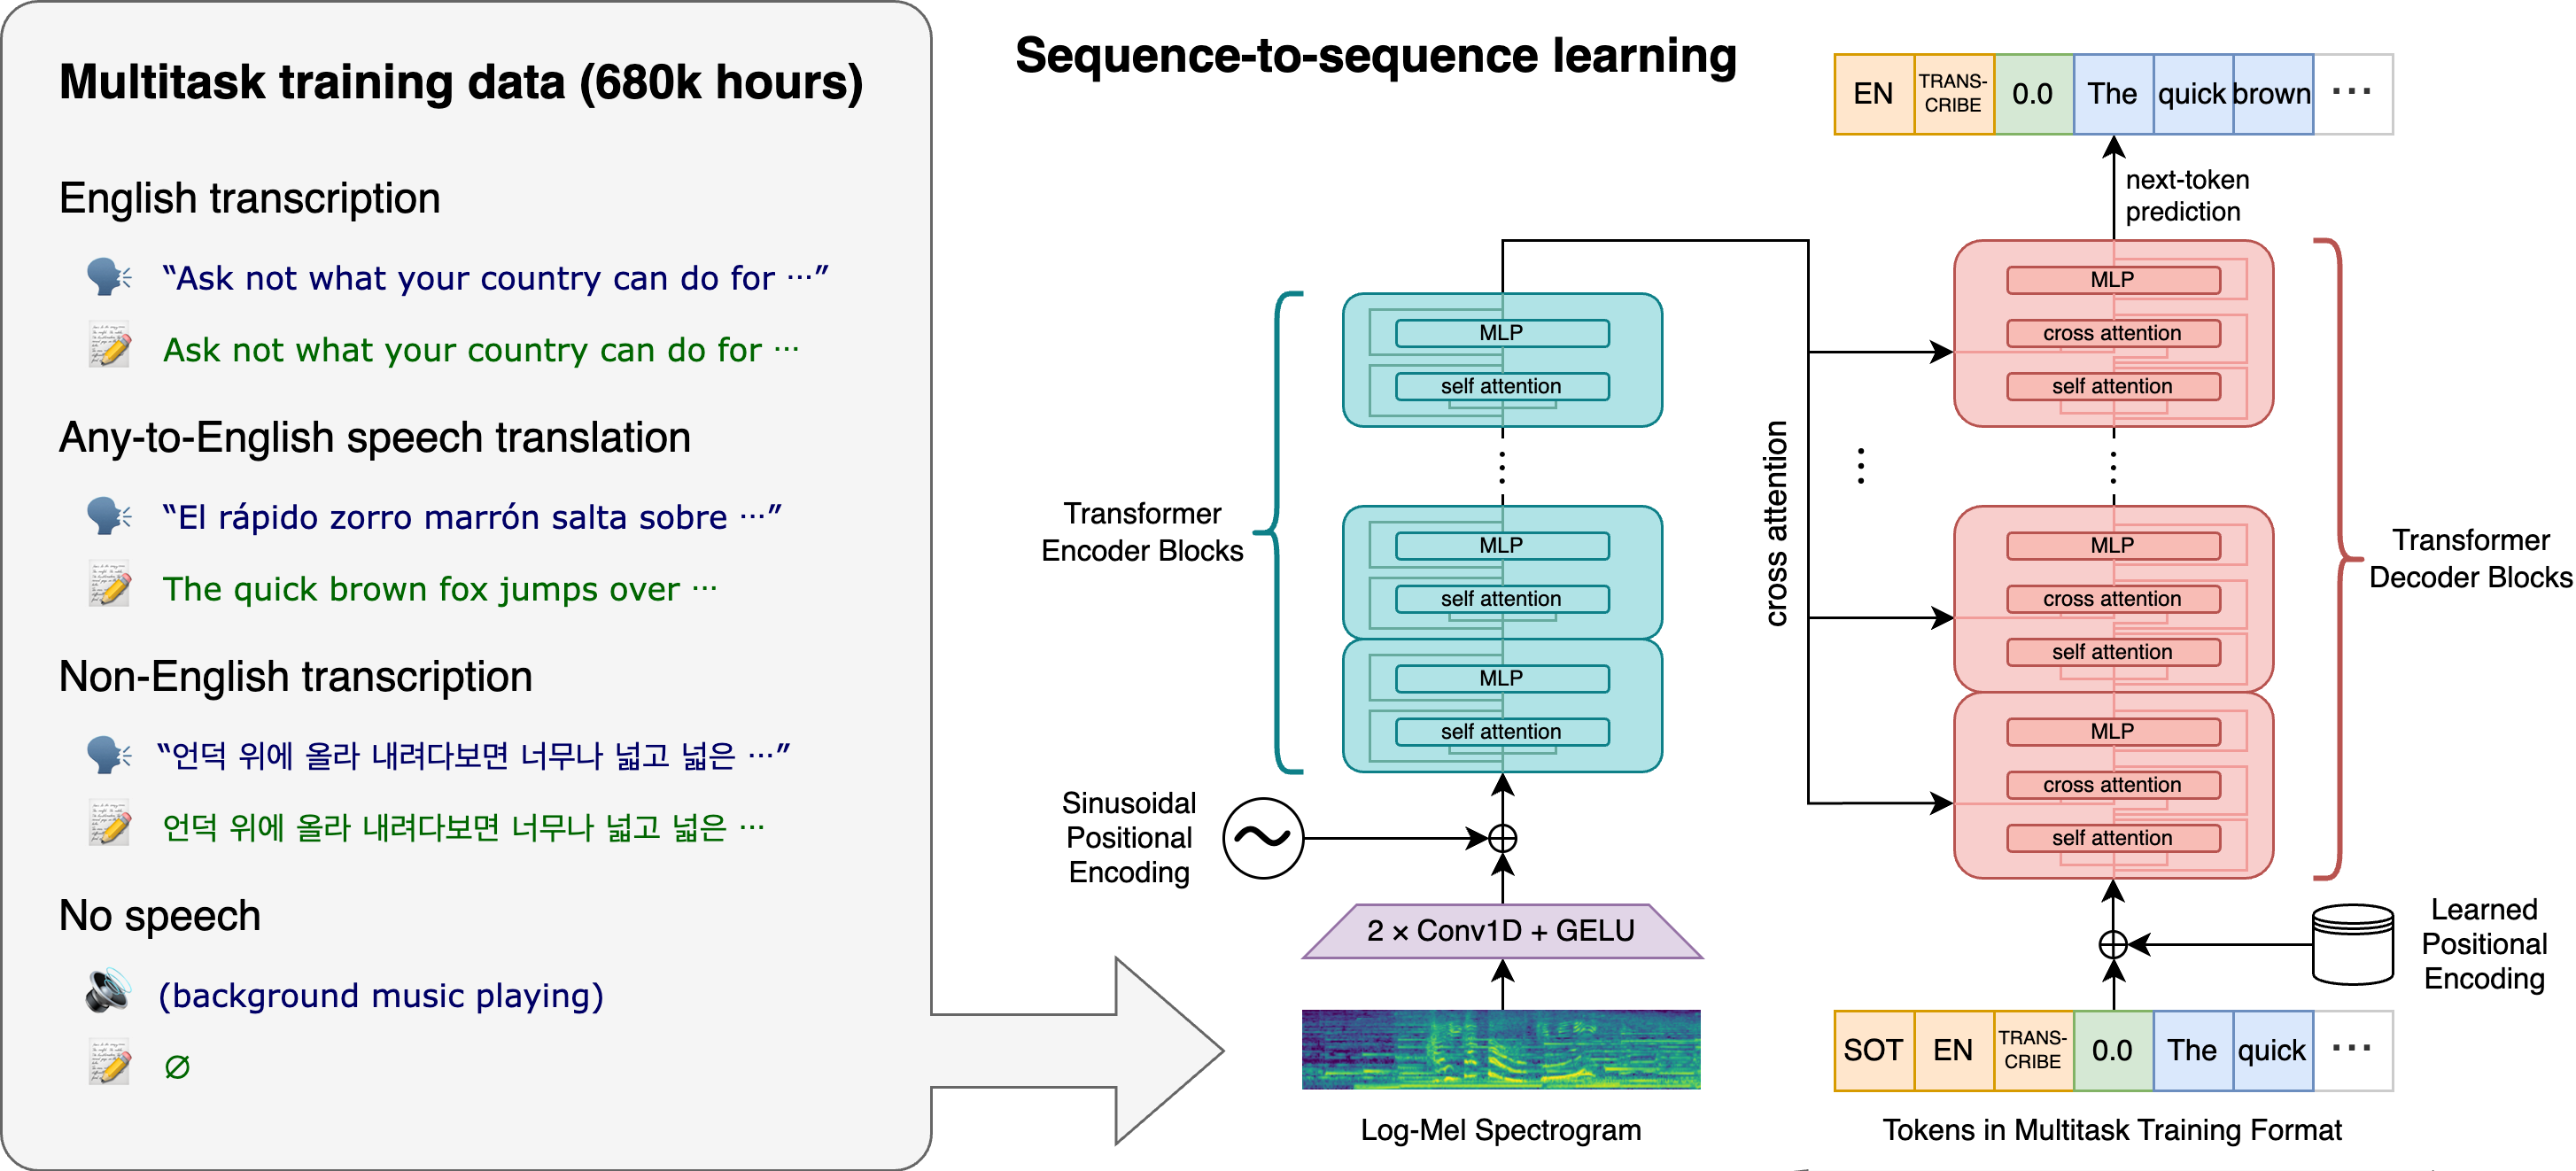
\includegraphics[width=13cm]{whisper_approach.png}};
	\end{tikzpicture}
	\vfill
	\lfr{Imagem: \url{https://github.com/openai/whisper}.}
	
\end{frame}
% ------------------------------------------------------------------------
\section{Encerramento}
\frame{
	\frametitle{Agradecimentos}
	\vspace{-0.25cm}
	\begin{figure}[h]
		\centering
		\subfloat[justification=Centering,singlelinecheck=false][]
		{\label{Fig_logo_icmg} 
\includegraphics[keepaspectratio,height=1.8cm]{LOGO_IC_CDR_12.pdf}}
	\end{figure}
	
	\begin{center}
		\textbf{Fim!}
	\end{center}
	\vspace{-0.25cm}
	\begin{small}
		Contatos:
		\begin{itemize}
			\item e-mail: adelinocpp@gmail.com, adelinocpp@yahoo.com ou adelino@ufmg.br;
			\item  Whatsapp (31) 98801-3605;
			\item Setor de Perícias em Áudio e Vídeo - Instituto de Criminalística. Av. Augusto de Lima, 1833, Barro Preto, Belo Horizonte-MG. Tel.: (31) 3330-1887;
			
		\end{itemize}        
	\end{small}
}
% ------------------------------------------------------------------------------
\begin{frame}[fragile=singleslide]
\frametitle{Sobre este material}
	Esta obra está licenciada sob a licença \href{http://creativecommons.org/licenses/by-nc-sa/4.0/}{\textit{Creative Commons} CC BY-NC-SA 4.0}\\
%	
	\flushleft
	Favor fazer referência a este trabalho como:\linebreak
	\begin{small}	
	Silva, A. P. (2023), \textit{Aplicação da Linguística Computacional nas Ciências Forenses}. Online: {\url{https://github.com/adelinocpp/estatistica-para-linguistica}}
	\linebreak
	\begin{addmargin}[0.5cm]{0em} 
		\begin{verbatim}
		@Misc{Silva2022,
		title={Aplicação da Linguística Computacional nas Ciências Forenses},
		author={Adelino Pinheiro Silva},
		howPublished={\url{https://github.com/adelinocpp/ada-lccf}},
		year={2022},
		note={Version 1.0; Creative Commons BY-NC-SA 4.0.},
		}
		\end{verbatim}
	\end{addmargin}
	\end{small}
	\vfill
	\begin{tikzpicture} [remember picture,overlay]
		\node[anchor=south,yshift=0.25cm] at (current page.south){ 
\includegraphics[width=.1\textwidth]{00BAS_CCsomerights.png}};
	\end{tikzpicture}
\end{frame} 
% ==============================================================================
\section{Dúvidas}
\begin{frame}[fragile=singleslide]
	\frametitle{Dúvidas}
	
		\begin{tikzpicture}[remember picture,overlay]
		\node[xshift=0cm,yshift=-0.5cm,opacity=1.0] at (current page.center) {\includegraphics[width=10cm]{principais-duvidas-sobre-o-trabalho-freelancer.jpg}};
	\end{tikzpicture}
	\vfill
	\lfr{Imagem: \url{https://www.hevcon.com.br/duvidas-frequentes-relacionado-ao-novo-bem-e-as-alteracoes-das-mps/}.}
	
\end{frame}
% ==============================================================================
\end{document}
